\chapter{Ongoing and Future Direction of PhD Research}

\label{ch:proposal}
In this chapter, we discuss the lines of research questions and the 

\subsection{Problem statement and Research Questions}

Modelling the behaviour of the legislator's behaviour and their support for legislation voting has attracted studies across political science and computer science. In the study of the ideal point, a legislators' ideological positions and preferences are estimated based on the historical voting patterns and behaviour. Ideal point estimation is a process of assigning a global representation of the legislator which has predictive and explanatory capabilities about the legislator. The ideal point estimation has attracted studies from political science \citep{Clinton2004, Clinton2012, feldman2013, heckman1997}, and from computer science \citep{Kraft, Kornilova,song, Gerrish2011}. The appeal of ideal point estimation manifest in two main ways. First, estimating ideal points provides \textit{descriptive} features for legislators and legislature bodies. Second, roll call models and ideal point estimates can be used for testing theories and prediction of legislative behaviour \cite{Clinton2004}. We focus on vote prediction problem: given the history of the legislator voting pattern, and the legislation text representation, can we predict the congressperson's vote? Along with this objective, we seek to find an optimal ideal representation, which demonstrates both descriptive and predictive features.

Figure \ref{fig:legistlativeVotingNetwork} demonstrates Legislative Voting Network as described in \cite{Gua}. In this setting, voters ($u$) and bills ($d$) are connected together based on the observed voting behaviour, and the associated link weight is either 1 ("Yea"), or -1 ("Nay"). Since each bill is made of mixture of words, we can speculate that the latent space between the bill textual representation and voting pattern contains descriptive and predictive features. In this content, we ignore the missing links (missing votes), and only focus on the observed voting behaviour. 

\begin{figure}[H]
\centering
\caption{Legislative voting network illustration}
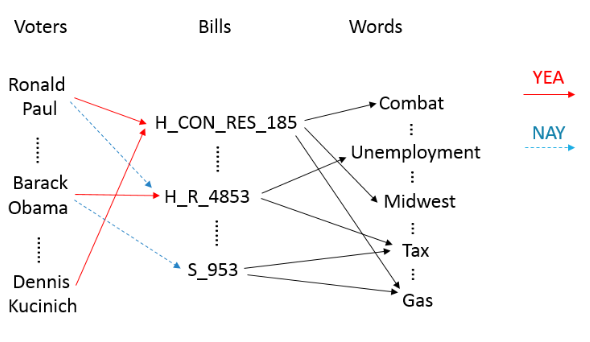
\includegraphics[scale=.5]{img/legistlativeVotingNetwork.png}
\label{fig:legistlativeVotingNetwork}
\end{figure}


To the best of our knowledge, most of the current research in legislators ideal point estimation and predictive models focuses on the United States legislative bodies. However, we intend to put more focus on the Canadian Parliament legislative behaviour, and examine the cross optimization of the models across different legislative bodies. To address some of the discussed issues, we propose taking our research direction to answer following research questions:

\begin{itemize}[noitemsep]
    \item (Bill Representation) How to best represent the legislation texts for predictive models across legislation bodies and time span. 
    \item (Legislator Representation) How to best extract the latent network space operating between the legislators.
    \item (Cross Optimization) Study the cross optimization of ideal points and predictive models across different legislative bodies. 
    \item (Neural Network - Ideal Points) How recent advances in NLP and Neural Network models can improve the ideal point estimations. 
\end{itemize}


\section{Related Work}


\subsection{Ideal Point Models}
The seminal contributions by \citet{pool_rosenthal_1985, pool_rosenthal_1991} are among the first attempts to model the legislative behaviour. There are Bayesian statistical modeling of the legislative behaviour and ideal point estimation developed by political scientist, notably by \citet{Clinton2004, Clinton2012}, \citet{heckman1997}. In another line of attempt to estimate ideal points, researcher employed topic models to represent the bill text \cite{Gerrish2011, Gua}. \citet{Gerrish2011} introduced an \textit{ideal point topic model} which applies a topic model similar to LDA \cite{Blei2003} to the bill text to estimate the legislator's ideal point. In later work, \citet{Gerrish2012HowTV} extended their approach to issue-adjusted ideal point to evaluate legislator's point for explicit topic related legislation. In this approach, legislators are also assigned topic adjusted position in addition to global ideal point. \citet{yano_tae_2012} and \citet{DBLP:journals/corr/abs-cs-0607062} analyzed transcripts of U.S. Congressional floor debates and bill text to predict whether speeches support or oppose the pending legislation, and whether a bill will survive the initial congressional committees.

In more recent attempts, \cite{Kraft} 

\subsection{Recommendation System and Collaborative Filtering}
The recommendation task in computer science domain can be considered to have a close objective to ideal point estimation models. In both tasks, researchers aim to estimate the latent factors that define the behaviour of the user/legislator. More specifically, given a user-item rating matrix, with user \textit{i} and item \textit{j}, entry at \textit{$i^{th}$} row and  \textit{$j^{th}$} column denotes the user rating of the item. The objective of the recommendation system in this case is to predict the item rating for users. Collaborative Filtering (CF) \cite{Herlocker:1999:AFP:312624.312682, Salakhutdinov:2007:RBM:1273496.1273596} and other matrix factorization based latent factor models \cite{koren_2009,Salakhutdinov:2007:PMF:2981562.2981720} have proved to be very successful at recommendation task. Non-Negative Matrix Factorization (NMF) \cite{Lee1999}, which we discussed as length in Section \ref{NMF}, is another successful latent factor model used in various context. 




\section{Our Approach}
\subsection{Models}

\section{Preliminary Comparative Study}
In previous sections, we described our objectives to 


\subsection{Legislation Dataset}
To best of our knowledge, there's no standard publicly available legislation dataset. However, most government legislative bodies have their data open to the open through their web portals. In the preliminary part of this project, we focus on the United States Congress, which includes both Senate and House of Representatives. Our dataset was collected from GovTrack \footnote{https://www.govtrack.us/}. We gathered roll call votes and texts of the bill introduced since the 106th congress to the most recent 115th congress. The dataset includes information about each legislator (personal information, party affiliation), complete bill text and information (sponsorship, date, category), and roll call information (final tally, date, participants). Table \ref{tab:legislationDataset} describe the overall information of our legislator dataset. Alternatively, Figure \ref{fig:congress-votes} shows the volume of votes per congress sessions.  


\begin{table}[htbp]
\centering
\begin{tabular}{l|lllllll}
\toprule
Congress & Years & President & House & Senate & Bills & Legislators & Votes \\
\midrule
106      &   1999-2001    & Clinton &   R   &   R     &  313  &  435 &  242,591  \\
107      &   2001-2003    & Bush    &   R   &   R     &  491  &  445 &  399,805  \\
108      &   2003-2005    & Bush    &   R   &   R     &  619  &  439 &  494,606  \\
109      &   2005-2007    & Bush    &   R   &   R     &  597  &  442 &  500,245  \\
110      &   2007-2009    & Bush    &   D   &   D     &  878  &  456 &  744,505  \\
111      &   2009-2011    & Obama   &   D   &   D     &  987  &  453 &  673,315  \\
112      &   2011-2013    & Obama   &   R   &   D     &  476  &  445 &  663,639  \\
113      &   2013-2015    & Obama   &   R   &   D     &  464  &  449 &  494,076  \\
114      &   2015-2017    & Obama   &   R   &   R     &  520  &  448 &  546,921  \\
115      &   2017-2019    & Trump   &   R   &   R     &  386  &  442 &  343,992  \\
\bottomrule
\end{tabular}
\caption{Legislation dataset stats}
\label{tab:legislationDataset}
\end{table}


\begin{figure}[H]
\centering
\caption{Volume of votes by each congress}
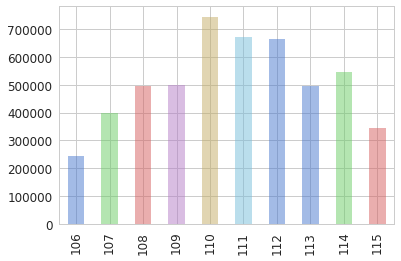
\includegraphics[scale=.7]{img/congress-votes.png}
\label{fig:congress-votes}
\end{figure}

It is important to analyze the Yea/Nay balance of the legislators dataset. Figure \ref{fig:congress-nay-yea} shows the class balance for each of congress session. As observed, most votes are cast Yea across all congress sessions. The rational behind this is that most bills will have the sponsored party support by the time they get to roll calls. 

\begin{figure}[H]
\centering
\caption{Volume of Yea/Nay votes by each congress}
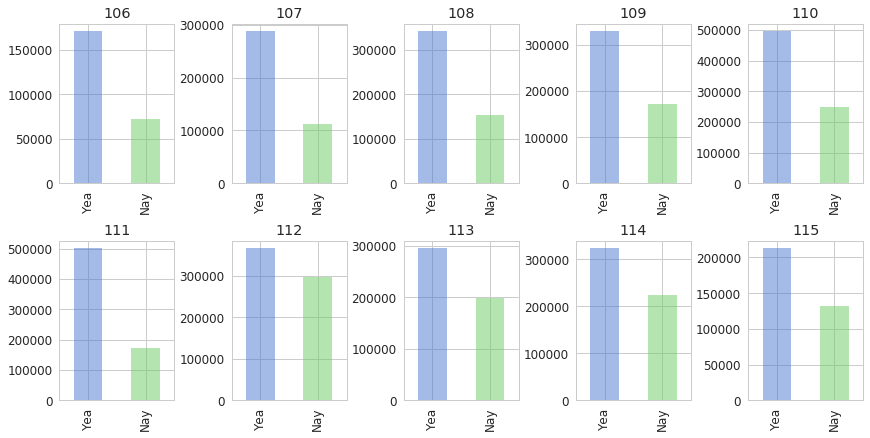
\includegraphics[scale=.55]{img/congress-nay-yea.png}
\label{fig:congress-nay-yea}
\end{figure}


\subsection{Pre-processing}
Following the gathering of the legislation dataset, we further process the dataset for the experiments. This task includes preprocessing the bill texts for machine learning consumption. We normalized the spaces, removed stop words and other domain related stop words, lemmatize the text to get more unified text for each bill. We also filter out any vote casts that are not on bills (such as votes for speaker of the house). The result of this process is two dataset, one holding all the voting records, and one holding all the bills. We use these two dataset and join them together for our machine learning experiments. 


\subsection{Experiments}


\subsection{Preliminary Results}

% \begin{tabular}{lrlrr}
% \toprule
% congress &    method & accuracy &             mse \\
% \midrule
% {} &  RandomForest &     0.719409 &       0.280591 \\
% 106 &  Majority & 0.702364 &       0.297636 \\
% {} &  Decision Tree &    0.719883 &  0.280117 \\
% 107 & 0.725704 &   RandomForest &         0.274296 \\
% 0.719876 &       Majority &       107 &  0.280124 \\
% 0.726342 &  Decision Tree &       107 &  0.273658 \\
% 0.698560 &   RandomForest &       108 &  0.301440 \\
% 0.690999 &       Majority &       108 &  0.309001 \\
% 0.698662 &  Decision Tree &       108 &  0.301338 \\
% 0.668243 &   RandomForest &       109 &  0.331757 \\
% 0.657418 &       Majority &       109 &  0.342582 \\
% 0.668303 &  Decision Tree &       109 &  0.331697 \\
% 0.682366 &   RandomForest &       110 &  0.317634 \\
% 0.662232 &       Majority &       110 &  0.337768 \\
% 0.682366 &  Decision Tree &       110 &  0.317634 \\
% 0.760187 &   RandomForest &       111 &  0.239813 \\
% 0.744377 &       Majority &       111 &  0.255623 \\
% 0.760127 &  Decision Tree &       111 &  0.239873 \\
% 0.608636 &   RandomForest &       112 &  0.391364 \\
% 0.549334 &       Majority &       112 &  0.450666 \\
% 0.608636 &  Decision Tree &       112 &  0.391364 \\
% 0.622602 &   RandomForest &       113 &  0.377398 \\
% 0.595572 &       Majority &       113 &  0.404428 \\
% 0.622470 &  Decision Tree &       113 &  0.377530 \\
% 0.617507 &   RandomForest &       114 &  0.382493 \\
% 0.591489 &       Majority &       114 &  0.408511 \\
% 0.617352 &  Decision Tree &       114 &  0.382648 \\
% 0.626928 &   RandomForest &       115 &  0.373072 \\
% 0.615314 &       Majority &       115 &  0.384686 \\
% 0.626724 &  Decision Tree &       115 &  0.373276 \\
% \bottomrule
% \end{tabular}

 
\begin{table*}[!ht]
\centering
  \caption{Classification performance results}
  \label{table:experimentalResult}
\resizebox{\textwidth}{!}{%
\begin{tabular}{lcccccccccccccccccccc}
\toprule
\textbf{Congress} & \multicolumn{2}{c}{\textbf{106}} & \multicolumn{2}{c}{\textbf{107}} &  \multicolumn{2}{c}{\textbf{108}} & \multicolumn{2}{c}{\textbf{110}} & \multicolumn{2}{c}{\textbf{111}} & \multicolumn{2}{c}{\textbf{112}} & \multicolumn{2}{c}{\textbf{113}}& \multicolumn{2}{c}{\textbf{114}} & \multicolumn{2}{c}{\textbf{115}} & \multicolumn{2}{c}{\textbf{116}} \\
\cmidrule(lr){2-21}
\textbf{Metric} & {acc} & {mse} & {acc} & {mse} & {acc} & {mse} & {acc} & {mse} & {acc} & {mse}  & {acc} & {mse}  & {acc} & {mse}  & {acc} & {mse}  & {acc} & {mse}   & {acc} & {mse}    \\
\midrule
\texttt{Majority}  &$0.579$ 	& $0.578$ & $0.954$ & $0.955$ &	$0.819$ & $0.819$ & $\textbf{0.813}$ & $0.747$ & $0.578$ & $0.954$ & $0.955$ &	$0.819$ & $0.819$ & $\textbf{0.813}$ & $0.747$ & $0.578$ & $0.954$ & $0.955$ &	$0.819$ & $0.819$ \\
\texttt{DT}  &$0.579$ 	& $0.578$ & $0.954$ & $0.955$ &	$0.819$ & $0.819$ & $\textbf{0.813}$ & $0.747$ & $0.578$ & $0.954$ & $0.955$ &	$0.819$ & $0.819$ & $\textbf{0.813}$ & $0.747$ & $0.578$ & $0.954$ & $0.955$ &	$0.819$ & $0.819$ \\

\midrule
\texttt{Conv}  &$0.579$ 	& $0.578$ & $0.954$ & $0.955$ &	$0.819$ & $0.819$ & $\textbf{0.813}$ & $0.747$ & $0.578$ & $0.954$ & $0.955$ &	$0.819$ & $0.819$ & $\textbf{0.813}$ & $0.747$ & $0.578$ & $0.954$ & $0.955$ &	$0.819$ & $0.819$ \\
\texttt{Meta}  &$0.579$ 	& $0.578$ & $0.954$ & $0.955$ &	$0.819$ & $0.819$ & $\textbf{0.813}$ & $0.747$ & $0.578$ & $0.954$ & $0.955$ &	$0.819$ & $0.819$ & $\textbf{0.813}$ & $0.747$ & $0.578$ & $0.954$ & $0.955$ &	$0.819$ & $0.819$ \\

\bottomrule             
\end{tabular}
}
\end{table*}



\section{Summary of Report Achievements}
In chapter 1, we present an interactive dialogue system that allows users to interact with a chatbot that is modelled on the political debates. This work includes natural language processing and generation techniques to generate dialogue responses to the user input. The goal of this work was to utilize the state-of-the-art generative neural networks and train them on political debate dataset and evaluate how the generative models operate in this domain-specific context. In chapter 2 we took an inquiry in understanding the fake news phenomena and evaluated various classification techniques on multiple curated datasets. The fake news has become a serious issue in political discourse, and yet it seems that the science to combat it has remained behind. The fake news classification task shows average performance, however, the availability of the representative dataset remains as an obstacle to combat fake news.

Lastly, we take a look at an effective topic modelling approach to analyze the news media to extract population displacements signals. We evaluate different topic modelling techniques and evaluate the topic coherence measures to find the best number of topics for a particular period. Based on this initial work, we further show that the violence related signals can be extracted from the dynamic topics, and can improve the population displacement prediction. 


\section{Future Plans}
Overall, this report focuses on the text analysis techniques, ranging from topic modelling, text classification, and text generation. These are three active research topics that open various lines of research for the future of my academic research. In future, I'm planning to expand on natural language analysis and modelling in the political science context. This work is encouraged by the availability of large political related data produced and available from government institutions and agencies. Analysis of the legislative voting rolls based on the content of the bills and the voting history of the legislator is an active research area that can benefit from state-of-the-art natural language understanding and classification techniques. 